\documentclass{report}

\input{~/dev/latex/template/preamble.tex}
\input{~/dev/latex/template/macros.tex}

\title{\Huge{}}
\author{\huge{Nathan Warner}}
\date{\huge{}}
\pagestyle{fancy}
\fancyhf{}
\lhead{Warner \thepage}
\rhead{}
% \lhead{\leftmark}
\cfoot{\thepage}
%\setborder
% \usepackage[default]{sourcecodepro}
% \usepackage[T1]{fontenc}

\begin{document}
    % \maketitle
        \begin{titlepage}
       \begin{center}
           \vspace*{1cm}
    
           \textbf{Calculus 2} \\
           Chapter 6
    
           \vspace{0.5cm}
            
                
           \vspace{1.5cm}
    
           \textbf{Nathan Warner}
    
           \vfill
                
                
           \vspace{0.8cm}
         
           
\includegraphics[width=0.4\textwidth]{~/niu/seal.png}
                
           Computer Science \\
           Northern Illinois University\\
           October 27, 2023 \\
           United States\\
           
                
       \end{center}
    \end{titlepage}
    \tableofcontents
    \pagebreak \bigbreak \noindent
    \vspace{2in} \\
    \begin{Huge}
       \textbf{Power Series} 
    \end{Huge}
    \bigbreak \noindent 
    \line(1,0){490}
    \bigbreak \noindent 
    \phantomsection
    \addcontentsline{toc}{section}{6.1 Power Series and Functions}
    \section*{6.1 Power Series and Functions}
    \bigbreak \noindent 
    A power series is a type of series with terms involving a variable. More specifically, if the variable is x, then all the terms of the series involve powers of x. As a result, a power series can be thought of as an infinite polynomial. Power series are used to represent common functions and also to define new functions. In this section we define power series and show how to determine when a power series converges and when it diverges. We also show how to represent certain functions using power series.
    \bigbreak \noindent 
    \phantomsection
    \addcontentsline{toc}{subsection}{Form of a Power Series}
    \subsection*{Form of a Power Series}
    \bigbreak \noindent 
    \begin{dfn}[Power series]
        A series of the form
    \begin{align*}
        \sum_{n=0}^{\infty} c_n x^n &= c_0 + c_1 x + c_2 x^2 + \cdots 
    .\end{align*}
    is a power series centered at \( x = 0 \).
    \bigbreak \noindent 
    A series of the form
    \begin{align*}
        \sum_{n=0}^{\infty} c_n (x - a)^n &= c_0 + c_1 (x - a) + c_2 (x - a)^2 + \cdots 
    .\end{align*}
    is a power series centered at \( x = a \).
    \end{dfn}
    
    \bigbreak \noindent 
    To make this definition precise, we stipulate that \( x^0 = 1 \) and \( (x - a)^0 = 1 \) even when \( x = 0 \) and \( x = a \), respectively.
    \bigbreak \noindent 
    The series
    \begin{align*}
        \sum_{n=0}^{\infty} \frac{x^n}{n!} &= 1 + x + \frac{x^2}{2!} + \frac{x^3}{3!} + \cdots
    \end{align*}
    and
    \begin{align*}
        \sum_{n=0}^{\infty} n! x^n &= 1 + x + 2! x^2 + 3! x^3 + \cdots
    \end{align*}
    are both power series centered at \( x = 0 \).
    \bigbreak \noindent 
    The series
    \begin{align*}
        \sum_{n=0}^{\infty} \frac{(x - 2)^n}{(n + 1)3^n} &= 1 + \frac{x - 2}{2 \cdot 3} + \frac{(x - 2)^2}{3 \cdot 3^2} + \frac{(x - 2)^3}{4 \cdot 3^3} + \cdots
    \end{align*}
    is a power series centered at \( x = 2 \).

    \bigbreak \noindent 
    \phantomsection
    \addcontentsline{toc}{subsection}{Convergence of a Power Series}
    \subsection*{Convergence of a Power Series}
    \bigbreak \noindent 
    \begin{thrmm}[Convergence of a Power Series]
        Consider the power series \(\sum_{n=0}^{\infty} c_n (x - a)^n\). The series satisfies exactly one of the following properties:
        \begin{enumerate}[label=(\roman*)]
            \item The series converges at \( x = a \) and diverges for all \( x \neq a \).
            \item The series converges for all real numbers \( x \).
            \item There exists a real number \( R > 0 \) such that the series converges if \( |x - a| < R \) and diverges if \( |x - a| > R \). At the values \( x \) where \( |x - a| = R \), the series may converge or diverge.
        \end{enumerate}
    \end{thrmm}
    \bigbreak \noindent 
    \begin{dfn}
        Consider the power series \(\sum_{n=0}^{\infty} c_n (x - a)^n\). The set of real numbers \( x \) where the series converges is the interval of convergence. If there exists a real number \( R > 0 \) such that the series converges for \( |x - a| < R \) and diverges for \( |x - a| > R \), then \( R \) is the radius of convergence. If the series converges only at \( x = a \), we say the radius of convergence is \( R = 0 \). If the series converges for all real numbers \( x \), we say the radius of convergence is \( R = \infty \) (Figure 6.2).
    \end{dfn}
    \bigbreak \noindent 
    \begin{center}
        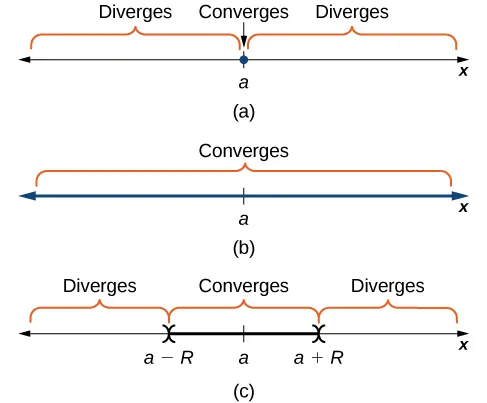
\includegraphics[scale=0.5]{./figures/popp.png}
    \end{center}

    \pagebreak \bigbreak \noindent 
    \begin{exm}
        Find the interval and radius of convergence
        \begin{align*}
            \summation{\infty}{n=1}\ \frac{x^{n}}{n!}\ 
        .\end{align*}
    \end{exm}
    \bigbreak \noindent 
    \textcolor{red}{\textit{Solution.}} For this, we use the ratio test and get
    \begin{align*}
        &\rho = \lim\limits_{n \to \infty}{\bigg\lvert \frac{\frac{x^{n}\cdot x}{n!(n+1)}}{\frac{n!}{x^{n}}} \bigg\rvert} \\
        &=\abs{x}\lim\limits_{n \to \infty}{\frac{1}{n+1}} \\
        &=0
    .\end{align*}
    \bigbreak \noindent 
    Since $ 0 \leq \rho  < 1$, this series will converge $\forall\ x \in \mathbb{R} $. Thus, the interval of convergence is $(-\infty,+\infty) $ and the radius of convergence is $R = \infty $

    \bigbreak \noindent 
    \begin{exm}
         Find the interval and radius of convergence
         \begin{align*}
             \summation{\infty}{n=0}\ n!x^{n}\ 
         .\end{align*}
    \end{exm}
    \bigbreak \noindent 
    \textcolor{red}{\textit{Solution.}} Again, we use the ratio test
    \begin{align*}
        &\rho = \lim\limits_{n \to \infty}{\frac{n!(n+1)x^{n}x}{n!x^{n}}} \\
        &=\abs{x}\lim\limits_{n \to \infty}{(n+1)} \\
        &=\infty
    .\end{align*}
    \bigbreak \noindent 
    Since $\rho = \infty $ The series diverges for all \( x \neq 0 \). Since the series is centered at \( x = 0 \), it must converge there, so the series converges only for \( x = 0 \). The interval of convergence is the single value \( x = 0 \) and the radius of convergence is \( R = 0 \).

    \pagebreak \bigbreak \noindent 
    \begin{exm}
        Find the interval and radius of convergence
        \begin{align*}
            \summation{\infty}{n=0}\ \frac{(x-2)^{n}}{(n+1)3^{n}}\ 
        .\end{align*}
    \end{exm}
    \bigbreak \noindent 
    \textcolor{red}{\textit{Solution.}} After applying the ratio test, we get
    \begin{align*}
        &\rho = \abs{x-2}\lim\limits_{n \to \infty}{\frac{n+1}{3n+2}} \\
        &=\frac{\abs{x-2}}{3}
    .\end{align*}
    \bigbreak \noindent 
    The question we ask is... when is this quantity $<1 $. 
    \begin{align*}
        &\frac{\abs{x-2}}{3} < 1 \\
        &\abs{x-2} < 3 \\
        &\implies -3 < x-2 < 3 \\
        &-1 < x < 5
    .\end{align*}
    \bigbreak \noindent 
    Thus, when $-1 < x < 5$, the series will converge absolutely. Likewise
    \begin{align*}
        &\frac{\abs{x-2}}{3} > 1 \\
        &\abs{x-2} > 3 \\
        \implies &x-2 < -3 \quad \text{ or } x-2 > 3 \\
        &x < -1 \quad \text{ or } x > 5
    .\end{align*}
    \bigbreak \noindent 
    Thus, the series will diverge if $x < -1$ or $x > 5$. Finally, we examine if $\rho = 1$
    \begin{align*}
        \frac{\abs{x-2}}{3} &= 1 \\
        \abs{x-2} &= 3 \\
        x-2 = 3 \quad &\quad x-2 = -3 \\
        x=5 \quad &\quad x=-1
    .\end{align*}
    \bigbreak \noindent 
    Thus, the ratio test is inconclusive for $x = -1$ or $x=5$. We need to test these values of $x$ separately. For $x=-1$ the series is given by
    \begin{align*}
        &\summation{\infty}{n=0}\ \frac{(-3)^{n}}{(n+1)3^{n}}\  \\
        &=\summation{\infty}{n=0}\ \frac{3^{n}(-1)^{n}}{(n+1)3^{n}}\  \\
        &=\summation{\infty}{n=0}\ \frac{(-1)^{n}}{n+1}\  
    .\end{align*}
    \bigbreak \noindent 
    Since this is the alternating harmonic series, it converges. Thus, the series converges at  $x=-1$. For $x=5$, the series is given by
    \begin{align*}
        &\summation{\infty}{n=0}\ \frac{3^{n}}{(n+1)3^{n}}\  \\
        &\summation{\infty}{n=0}\ \frac{1}{n+1}\ 
    .\end{align*}
    This is the harmonic series, which is divergent. Therefore, the power series diverges at \( x = 5 \). We conclude that the interval of convergence is \([ -1, 5 )\) and the radius of convergence is \( R = 3 \).

    \bigbreak \noindent 
    \phantomsection
    \addcontentsline{toc}{subsection}{Representing Functions as Power Series}
    \subsection*{Representing Functions as Power Series}
    \bigbreak \noindent 
    Being able to represent a function by an “infinite polynomial” is a powerful tool. Polynomial functions are the easiest functions to analyze, since they only involve the basic arithmetic operations of addition, subtraction, multiplication, and division. If we can represent a complicated function by an infinite polynomial, we can use the polynomial representation to differentiate or integrate it. In addition, we can use a truncated version of the polynomial expression to approximate values of the function. So, the question is, when can we represent a function by a power series?
    \bigbreak \noindent 
    Consider again the geometric series
\begin{equation}
    1 + x + x^2 + x^3 + \cdots = \sum_{n=0}^{\infty} x^n 
\end{equation}
Recall that the geometric series
\[
    a + ar + ar^2 + ar^3 + \cdots
\]
converges if and only if \( |r| < 1 \). In that case, it converges to \(\frac{a}{1 - r}\). Therefore, if \( |x| < 1 \), the series in Example 6.3 converges to \(\frac{1}{1 - x}\) and we write
\[
    1 + x + x^2 + x^3 + \cdots = \frac{1}{1 - x} \quad \text{for} \quad |x| < 1.
\]
As a result, we are able to represent the function \( f(x) = \frac{1}{1 - x} \) by the power series
\[
    1 + x + x^2 + x^3 + \cdots \quad \text{when} \quad |x| < 1.
\]
We now show graphically how this series provides a representation for the function \( f(x) = \frac{1}{1 - x} \) by comparing the graph of \( f \) with the graphs of several of the partial sums of this infinite series.

    \bigbreak \noindent 
    \begin{exm}
       Use a power series to represent each of the following functions  $f$. Find the interval of convergence. 
       \begin{align*}
           f(x) = \frac{1}{1+x^{3}}
       .\end{align*}
    \end{exm}
    \bigbreak \noindent 
    \textcolor{red}{\textit{Solution.}} should recognize this function $f$ as the sum of a geometric series, because
    \begin{align*}
        \frac{1}{1+x^{3}} = \frac{1}{1-(-x^{3})}
    .\end{align*}
    Using the fact that, for \( |r| < 1 \), \(\frac{a}{1 - r}\) is the sum of the geometric series
\[
    \sum_{n=0}^{\infty} ar^n = a + ar + ar^2 + \cdots,
\]
we see that, for \( \left| -x^3 \right| < 1 \),
\[
    \frac{1}{1 + x^3} = \frac{1}{1 - (-x^3)} = \sum_{n=0}^{\infty} (-x^3)^n = 1 - x^3 + x^6 - x^9 + \cdots.
\]
Since this series converges if and only if \( \left| -x^3 \right| < 1 \), the interval of convergence is \( (-1, 1) \), and we have
\[
    \frac{1}{1 + x^3} = 1 - x^3 + x^6 - x^9 + \cdots \quad \text{for} \quad |x| < 1.
\]


    \pagebreak \bigbreak \noindent 
    \begin{exm}
       Use a power series to represent each of the following functions  $f$. Find the interval of convergence. 
       \begin{align*}
           \summation{\infty}{n=0}\ \frac{x^{2}}{4-x^{2}}\ 
       .\end{align*}
    \end{exm}
    \bigbreak \noindent 
    This function is not in the exact form of a sum of a geometric series. However, with a little algebraic manipulation, we can relate \( f \) to a geometric series. By factoring \( 4 \) out of the two terms in the denominator, we obtain
    \[
        \frac{x^2}{4 - x^2} = \frac{x^2}{4(1 - \frac{x^2}{4})} = \frac{x^2}{4}\left(1 - \left(\frac{x^2}{2}\right)^2\right).
    \]
    \bigbreak \noindent 
    Therefore, we have
    \[
        \frac{x^2}{4 - x^2} = \frac{x^2}{4}\left(1 - \left(\frac{x^2}{2}\right)^2\right) = \frac{x^2}{4}\frac{1}{1 - \left(\frac{x^2}{2}\right)^2} = \sum_{n=0}^{\infty} \frac{x^2}{4}\left(\frac{x^2}{2}\right)^{2n}.
    \]
    \bigbreak \noindent 
    The series converges as long as \( \left|\left(\frac{x^2}{2}\right)^2\right| < 1 \) (note that when \( \left|\left(\frac{x^2}{2}\right)^2\right| = 1 \) the series does not converge). Solving this inequality, we conclude that the interval of convergence is \( (-2, 2) \), and
    \[
        \frac{x^2}{4 - x^2} = \sum_{n=0}^{\infty} \frac{x^{2n?2}}{4^{n+1}} = \frac{x^2}{4} + \frac{x^4}{4^2} + \frac{x^6}{4^3} + \cdots
    \]
    \bigbreak \noindent 
    for \( |x| < 2 \).

    \pagebreak \bigbreak \noindent 
    \phantomsection
    \addcontentsline{toc}{section}{6.2 Properties of Power Series}
    \section*{6.2 Properties of Power Series}
    \bigbreak \noindent 
    \phantomsection
    \addcontentsline{toc}{subsection}{Combining Power Series}
    \subsection*{Combining Power Series}
    \bigbreak \noindent 
    If we have two power series with the same interval of convergence, we can add or subtract the two series to create a new power series, also with the same interval of convergence. Similarly, we can multiply a power series by a power of \( x \) or evaluate a power series at \( x^m \) for a positive integer \( m \) to create a new power series. Being able to do this allows us to find power series representations for certain functions by using power series representations of other functions. For example, since we know the power series representation for \( f(x) = \frac{1}{1-x} \), we can find power series representations for related functions, such as \ldots

    \bigbreak \noindent 

    \begin{thrmm}[Combining Power Series]
        Suppose that the two power series \(\sum_{n=0}^{\infty} c_n x^n\) and \(\sum_{n=0}^{\infty} d_n x^n\) converge to the functions \(f\) and \(g\), respectively, on a common interval \(I\).
    \begin{enumerate}[label=(\roman*)]
        \item The power series \(\sum_{n=0}^{\infty} (c_n x^n \pm d_n x^n)\) converges to \(f \pm g\) on \(I\).
        \item For any integer \(m \geq 0\) and any real number \(b\), the power series \(\sum_{n=0}^{\infty} b x^m c_n x^n\) converges to \(b x^m f(x)\) on \(I\).
        \item For any integer \(m \geq 0\) and any real number \(b\), the series \(\sum_{n=0}^{\infty} c_n (b x^m)^n\) converges to \(f(b x^m)\) for all \(x\) such that \(b x^m\) is in \(I\).
    \end{enumerate}
    \end{thrmm}

    \bigbreak \noindent 
    \begin{exm}
       Suppose that \(\sum_{n=0}^{\infty} a_n x^n\) is a power series whose interval of convergence is \((-1, 1)\), and suppose that \(\sum_{n=0}^{\infty} b_n x^n\) is a power series whose interval of convergence is \((-2, 2)\).
       \bigbreak \noindent 
       Find the interval of convergence of the series \(\sum_{n=0}^{\infty} (a_n x^n + b_n x^n)\).
    \end{exm}
    \bigbreak \noindent 
    \textcolor{red}{\textit{Solution.}} Since the interval \((-1, 1)\) is a common interval of convergence of the series \(\sum_{n=0}^{\infty} a_n x^n\) and \(\sum_{n=0}^{\infty} b_n x^n\), the interval of convergence of the series \(\sum_{n=0}^{\infty} (a_n x^n + b_n x^n)\) is \((-1, 1)\).

    \bigbreak \noindent 
    \begin{exm}
        Suppose that \(\sum_{n=0}^{\infty} a_n x^n\) is a power series whose interval of convergence is \((-1, 1)\), and suppose that \(\sum_{n=0}^{\infty} b_n x^n\) is a power series whose interval of convergence is \((-2, 2)\).
        \bigbreak \noindent 
        Find the interval of convergence of the series \(\sum_{n=0}^{\infty} a_n 3^n x^n\).
    \end{exm}
    \bigbreak \noindent 
    \textcolor{red}{\textit{Solution.}} Since \(\sum_{n=0}^{\infty} a_n x^n\) is a power series centered at zero with radius of convergence 1, it converges for all \(x\) in the interval \((-1, 1)\). By combining power series, the series \(\sum_{n=0}^{\infty} a_n 3^n x^n = \sum_{n=0}^{\infty} a_n (3x)^n\) converges if \(3x\) is in the interval \((-1, 1)\). Therefore, the series converges for all \(x\) in the interval \(\left(-\frac{1}{3}, \frac{1}{3}\right)\).

    \pagebreak \bigbreak \noindent 
    In the next example, we show how to use Combining Power Series and the power series for a function \( f \) to construct power series for functions related to \( f \). Specifically, we consider functions related to the function \( f(x) = \frac{1}{1 - x} \) and we use the fact that
    \[
    \frac{1}{1 - x} = \sum_{n=0}^{\infty} x^n = 1 + x + x^2 + x^3 + \cdots
    \]
    for \( |x| < 1 \)

    \bigbreak \noindent 
    \begin{exm}[Constructing Power Series from Known Power Series]
        Use the power series representation for \( f(x) = \frac{1}{1 - x} \) combined with Combining Power Series to construct a power series for each of the following functions. Find the interval of convergence of the power series.
        \begin{align*}
            f(x) = \frac{3x}{1+x^{2}}
        .\end{align*}
        
    \end{exm}
    \bigbreak \noindent 
    \textcolor{red}{\textit{Solution.}} First write \( f(x) \) as
    \[ f(x) = 3x \left( \frac{1}{1 - (-x^2)} \right). \]
    Using the power series representation for \( f(x) = \frac{1}{1 - x} \) and parts ii. and iii. of Combining Power Series, we find that a power series representation for \( f \) is given by
    \[ \sum_{n=0}^{\infty} 3x(-x^2)^n = \sum_{n=0}^{\infty} 3(-1)^n x^{2n+1}. \]
    Since the interval of convergence of the series for \( \frac{1}{1 - x} \) is \((-1, 1)\), the interval of convergence for this new series is the set of real numbers \( x \) such that \( |x^2| < 1 \). Therefore, the interval of convergence is \((-1, 1)\).

    \bigbreak \noindent 
    \begin{exm}[Constructing Power Series from Known Power Series]
        Use the power series representation for \( f(x) = \frac{1}{1 - x} \) combined with Combining Power Series to construct a power series for each of the following functions. Find the interval of convergence of the power series.
        \begin{align*}
            f(x)  =\frac{1}{(x-1)(x-3)}
        .\end{align*}
    \end{exm}
    \bigbreak \noindent 
    \textcolor{red}{\textit{Solution.}}
    To find the power series representation, use partial fractions to write \( f(x) = \frac{1}{(x-1)(x-3)} \) as the sum of two fractions. We have
    \begin{align*}
        &\frac{1}{(x-1)(x-3)}  \\
        =&-\frac{1}{2(x-1)} + \frac{1}{2(x-3)} \\
        =&\frac{1}{2(1-x)} - \frac{1}{6(1-\frac{x}{3})}
    .\end{align*}
    First, using part ii. of Combining Power Series, we obtain
    \[
    \frac{1}{2(1-x)} = \sum_{n=0}^{\infty} \frac{1}{2} x^n \text{ for } |x| < 1.
    \]
    Then, using parts ii. and iii. of Combining Power Series, we have
    \[
    \frac{1}{6(1-\frac{x}{3})} = \sum_{n=0}^{\infty} \frac{1}{6} \left(\frac{x}{3}\right)^n \text{ for } |x| < 3.
    \]
    Since we are combining these two power series, the interval of convergence of the difference must be the smaller of these two intervals. Using this fact and part i. of Combining Power Series, we have
    \[
    \frac{1}{(x-1)(x-3)} = \sum_{n=0}^{\infty} \left(\frac{1}{2} - \frac{1}{6} \cdot 3^n\right) x^n
    \]
    where the interval of convergence is \((-1,1)\).

    \bigbreak \noindent 
    Now we try the opposite... Given a power series, determine which function it represents.
    \bigbreak \noindent 
    \begin{exm}[Finding the Function Represented by a Given Power Series]
        Consider the power series \(\sum_{n=0}^{\infty} 2^n x^n\). Find the function \( f \) represented by this series. Determine the interval of convergence of the series.
    \end{exm}

    \bigbreak \noindent 
    \phantomsection
    \addcontentsline{toc}{subsection}{Multiplication of Power Series}
    \subsection*{Multiplication of Power Series}
    \bigbreak \noindent 
    We can also create new power series by multiplying power series. Being able to multiply two power series provides another way of finding power series representations for functions.
    \bigbreak \noindent 
    The way we multiply them is similar to how we multiply polynomials. For example, suppose we want to multiply
    \[
    \sum_{n=0}^{\infty} c_n x^n = c_0 + c_1 x + c_2 x^2 + \cdots
    \]
    and
    \[
    \sum_{n=0}^{\infty} d_n x^n = d_0 + d_1 x + d_2 x^2 + \cdots.
    \]
    It appears that the product should satisfy
    \begin{align*}
        \left( \sum_{n=0}^{\infty} c_n x^n \right) \left( \sum_{n=0}^{\infty} d_n x^n \right) &= (c_0 + c_1 x + c_2 x^2 + \cdots) \cdot (d_0 + d_1 x + d_2 x^2 + \cdots)  \\
        &= c_0 d_0 + (c_1 d_0 + c_0 d_1) x + (c_2 d_0 + c_1 d_1 + c_0 d_2) x^2 + \cdots.
    .\end{align*}
    In Multiplying Power Series, we state the main result regarding multiplying power series, showing that if \(\sum_{n=0}^{\infty} c_n x^n\) and \(\sum_{n=0}^{\infty} d_n x^n\) converge on a common interval \(I\), then we can multiply the series in this way, and the resulting series also converges on the interval \(I\).
    \pagebreak \bigbreak \noindent 
    \begin{thrmm}[Multiplying Power Series]
        Suppose that the power series \(\sum_{n=0}^{\infty} c_n x^n\) and \(\sum_{n=0}^{\infty} d_n x^n\) converge to \(f\) and \(g\), respectively, on a common interval \(I\). Let
        \begin{align*}
            &e_n = c_0 d_n + c_1 d_{n-1} + c_2 d_{n-2} + \cdots + c_{n-1} d_1 + c_n d_0  \\
            &= \sum_{k=0}^{n} c_k d_{n-k}.
        .\end{align*}
        Then
        \[
        \left( \sum_{n=0}^{\infty} c_n x^n \right) \left( \sum_{n=0}^{\infty} d_n x^n \right) = \sum_{n=0}^{\infty} e_n x^n
        \]
        and
        \[
        \sum_{n=0}^{\infty} e_n x^n \text{ converges to } f(x) \cdot g(x) \text{ on } I.
        \]
        The series \(\sum_{n=0}^{\infty} e_n x^n\) is known as the Cauchy product of the series \(\sum_{n=0}^{\infty} c_n x^n\) and \(\sum_{n=0}^{\infty} d_n x^n\).
    \end{thrmm}
    \bigbreak \noindent 
    \begin{exm}
        Multiply the power series representation
        \[
        \frac{1}{1 - x} = \sum_{n=0}^{\infty} x^n = 1 + x + x^2 + x^3 + \cdots
        \]
        for \( |x| < 1 \) with the power series representation
        \[
        \frac{1}{1 - x^2} = \sum_{n=0}^{\infty} (x^2)^n = 1 + x^2 + x^4 + x^6 + \cdots
        \]
        for \( |x| < 1 \) to construct a power series for \( f(x) = \frac{1}{(1 - x)(1 - x^2)} \) on the interval \( (-1, 1) \).
    \end{exm}
    \bigbreak \noindent 
    \textcolor{red}{\textit{Solution.}} 
    We need to multiply
    \[
    (1 + x + x^2 + x^3 + \cdots)(1 + x^2 + x^4 + x^6 + \cdots).
    \]
    Writing out the first several terms, we see that the product is given by
    \[
    \begin{aligned}
    &(1 + x^2 + x^4 + x^6 + \cdots) + (x + x^3 + x^5 + x^7 + \cdots) + \\
    &(x^2 + x^4 + x^6 + x^8 + \cdots) + (x^3 + x^5 + x^7 + x^9 + \cdots) \\
    &= 1 + x + (1 + 1)x^2 + (1 + 1)x^3 + (1 + 1 + 1)x^4 + (1 + 1 + 1)x^5 + \cdots \\
    &= 1 + x + 2x^2 + 2x^3 + 3x^4 + 3x^5 + \cdots.
    \end{aligned}
    \]
    Since the series for \( y = \frac{1}{1 - x} \) and \( y = \frac{1}{1 - x^2} \) both converge on the interval \( (-1, 1) \), the series for the product also converges on the interval \( (-1, 1) \).


    \pagebreak 
    \phantomsection
    \addcontentsline{toc}{subsection}{Differentiating and Integrating Power Series}
    \subsection*{Differentiating and Integrating Power Series}
    \bigbreak \noindent 
    \begin{thrmm}[Term-by-Term Differentiation and Integration for Power Series]
         Suppose that the power series $\sum_{n=0}^{\infty} c_n (x - a)^n$ converges on the interval $(a - R, a + R)$ for some $R > 0$. Let $f$ be the function defined by the series
        \[
        f(x) = \sum_{n=0}^{\infty} c_n (x - a)^n = c_0 + c_1(x - a) + c_2(x - a)^2 + c_3(x - a)^3 + \cdots
        \]
        for $|x - a| < R$. Then $f$ is differentiable on the interval $(a - R, a + R)$ and we can find $f'$ by differentiating the series term-by-term:
        \[
        f'(x) = \sum_{n=1}^{\infty} n c_n (x - a)^{n-1} = c_1 + 2c_2(x - a) + 3c_3(x - a)^2 + \cdots
        \]
        for $|x - a| < R$. Also, to find $\int f(x) \, dx$, we can integrate the series term-by-term. The resulting series converges on $(a - R, a + R)$, and we have
        \[
        \int f(x) \, dx = C + \sum_{n=0}^{\infty} \frac{c_n (x - a)^{n+1}}{n+1} = C + c_0(x - a) + \frac{c_1(x - a)^2}{2} + \frac{c_2(x - a)^3}{3} + \cdots
        \]
        for $|x - a| < R$.
        \bigbreak \noindent 
        \textbf{NOTE!} when a power series is differentiated or integrated term-by-term, it says nothing about what happens at the endpoints.
    \end{thrmm}

    \bigbreak \noindent 
    \begin{exm}
        Use the power series representation
        \[ f(x) = \frac{1}{1-x} = \sum_{n=0}^{\infty} x^n = 1 + x + x^2 + x^3 + \cdots \]
        for \( |x| < 1 \) to find a power series representation for
        \[ g(x) = \frac{1}{(1-x)^2} \]
        on the interval \( (-1,1) \). Determine whether the resulting series converges at the endpoints.
        \bigbreak \noindent 
        Use the result to evaluate the sum of the series 
        \[ \sum_{n=0}^{\infty} \frac{n+1}{4^n}. \]
    \end{exm}

    \pagebreak \bigbreak \noindent 
    \textcolor{red}{\textit{Solution.}} Since \( g(x) = \frac{1}{(1-x)^2} \) is the derivative of \( f(x) = \frac{1}{1-x} \), we can find a power series representation for \( g \) by differentiating the power series for \( f \) term-by-term. The result is
    \begin{align*}
         &g(x) = \frac{1}{(1-x)^2} \\
         &= \frac{d}{dx}\left(\frac{1}{1-x}\right) \\
         &= \sum_{n=0}^{\infty} \frac{d}{dx}(x^n) \\
         &= \frac{d}{dx}(1 + x + x^2 + x^3 + \cdots) \\
         &= 0 + 1 + 2x + 3x^2 + 4x^3 + \cdots \\
         &= \sum_{n=0}^{\infty} (n+1)x^n 
    .\end{align*}
    for \( |x| < 1 \). Term-by-Term Differentiation and Integration for Power Series does not guarantee anything about the behavior of this series at the endpoints. Testing the endpoints by using the divergence test, we find that the series diverges at both endpoints \( x = \pm 1 \).
    Note that this is the same result found in Example 6.8.
    \bigbreak \noindent 
    From part a. we know that
    \[ \sum_{n=0}^{\infty} (n+1)x^n = \frac{1}{(1-x)^2}. \]
    Therefore,
    \begin{align*}
         &\sum_{n=0}^{\infty} \frac{n+1}{4^n}  \\
         &= \sum_{n=0}^{\infty} (n+1)\left(\frac{1}{4}\right)^n  \\
         &= \frac{1}{\left(1-\frac{1}{4}\right)^2}  \\
         &= \frac{1}{\left(\frac{3}{4}\right)^2}  \\
         &= \frac{16}{9}. 
    .\end{align*}

    \bigbreak \noindent 
    \begin{thrmm}[Uniqueness of Power Series]
        Let $\sum_{n=0}^{\infty} c_n (x - a)^n$ and $\sum_{n=0}^{\infty} d_n (x - a)^n$ be two convergent power series such that
        \[
        \sum_{n=0}^{\infty} c_n (x - a)^n = \sum_{n=0}^{\infty} d_n (x - a)^n
        \]
        for all \( x \) in an open interval containing \( a \). Then \( c_n = d_n \) for all \( n \geq 0 \).
    \end{thrmm}

    \pagebreak 
    \phantomsection
    \addcontentsline{toc}{section}{6.3 Taylor and Maclaurin Series}
    \section*{6.3 Taylor and Maclaurin Series}
    \bigbreak \noindent 
    Consider a function $f$ that has a power series representation at $x=a$. Then the series has the form
    \begin{equation}
        \sum_{n=0}^{\infty} c_n(x-a)^n = c_0 + c_1(x-a) + c_2(x-a)^2 + \cdots.
    \end{equation}
    (6.4)
    What should the coefficients be? For now, we ignore issues of convergence, but instead focus on what the series should be, if one exists. We return to discuss convergence later in this section. If the series Equation 6.4 is a representation for $f$ at $x=a$, we certainly want the series to equal $f(a)$ at $x=a$. Evaluating the series at $x=a$, we see that
    \begin{equation}
        \sum_{n=0}^{\infty} c_n(x-a)^n = c_0 + c_1(a-a) + c_2(a-a)^2 + \cdots = c_0.
    \end{equation}
    Thus, the series equals $f(a)$ if the coefficient $c_0 = f(a)$. In addition, we would like the first derivative of the power series to equal $f'(a)$ at $x=a$. Differentiating Equation 6.4 term-by-term, we see that
    \begin{equation}
        \frac{d}{dx}\left(\sum_{n=0}^{\infty} c_n(x-a)^n\right) = c_1 + 2c_2(x-a) + 3c_3(x-a)^2 + \cdots.
    \end{equation}
    Therefore, at $x=a$, the derivative is
    \begin{equation}
        \frac{d}{dx}\left(\sum_{n=0}^{\infty} c_n(x-a)^n\right) = c_1 + 2c_2(a-a) + 3c_3(a-a)^2 + \cdots = c_1.
    \end{equation}
    Therefore, the derivative of the series equals $f'(a)$ if the coefficient $c_1 = f'(a)$. Continuing in this way, we look for coefficients $c_n$ such that all the derivatives of the power series Equation 6.4 will agree with all the corresponding derivatives of $f$ at $x=a$. The second and third derivatives of Equation 6.4 are given by
    \begin{equation}
        \frac{d^2}{dx^2}\left(\sum_{n=0}^{\infty} c_n(x-a)^n\right) = 2c_2 + 3 \cdot 2c_3(x-a) + 4 \cdot 3c_4(x-a)^2 + \cdots
    \end{equation}
    and
    \begin{equation}
        \frac{d^3}{dx^3}\left(\sum_{n=0}^{\infty} c_n(x-a)^n\right) = 3 \cdot 2c_3 + 4 \cdot 3 \cdot 2c_4(x-a) + 5 \cdot 4 \cdot 3c_5(x-a)^2 + \cdots.
    \end{equation}
    Therefore, at $x=a$, the second and third derivatives
    \begin{equation}
        \frac{d^2}{dx^2}\left(\sum_{n=0}^{\infty} c_n(x-a)^n\right) = 2c_2 + 3 \cdot 2c_3(a-a) + 4 \cdot 3c_4(a-a)^2 + \cdots = 2c_2
    \end{equation}
    and
    \begin{equation}
        \frac{d^3}{dx^3}\left(\sum_{n=0}^{\infty} c_n(x-a)^n\right) = 3 \cdot 2c_3 + 4 \cdot 3 \cdot 2c_4(a-a) + 5 \cdot 4 \cdot 3c_5(a-a)^2 + \cdots = 3 \cdot 2c_3
    \end{equation}
    equal $f''(a)$ and $f'''(a)$, respectively, if $c_2 = \frac{f''(a)}{2}$ and $c_3 = \frac{f'''(a)}{3 \cdot 2}$. More generally, we see that if $f$ has a power series representation at $x=a$, then the coefficients should be given by $c_n = \frac{f^{(n)}(a)}{n!}$. That is, the series should be
    \begin{equation}
        \sum_{n=0}^{\infty} \frac{f^{(n)}(a)}{n!}(x-a)^n = f(a) + f'(a)(x-a) + \frac{f''(a)}{2!}(x-a)^2 + \frac{f'''(a)}{3!}(x-a)^3 + \cdots.
    \end{equation}
    This power series for $f$ is known as the Taylor series for $f$ at $a$. If $a=0$, then this series is known as the Maclaurin series for $f$.
    \pagebreak 
    \begin{dfn}[Taylor-Maclaurin Series]
        If $f$ has derivatives of all orders at $x=a$, then the Taylor series for the function $f$ at $a$ is
        \begin{equation}
            \sum_{n=0}^{\infty} \frac{f^{(n)}(a)}{n!}(x-a)^n = f(a) + f'(a)(x-a) + \frac{f''(a)}{2!}(x-a)^2 + \cdots + \frac{f^{(n)}(a)}{n!}(x-a)^n + \cdots.
        \end{equation}
        The Taylor series for $f$ at $0$ is known as the Maclaurin series for $f$.
    \end{dfn}
    \begin{thrmm}[Uniqueness of Taylor series]
        If a function $f$ has a power series at $a$ that converges to $f$ on some open interval containing $a$, then that power series is the Taylor series for $f$ at $a$.
    \end{thrmm}
    \bigbreak \noindent 
    \phantomsection
    \addcontentsline{toc}{subsection}{Taylor Polynomials}
    \subsection*{Taylor Polynomials}
    \begin{dfn}[Taylor-Maclaurin Polynomial]
        If $f$ has $n$ derivatives at $x=a$, then the $n$th Taylor polynomial for $f$ at $a$ is
        \begin{equation}
            p_n(x) = f(a) + f'(a)(x-a) + \frac{f''(a)}{2!}(x-a)^2 + \frac{f'''(a)}{3!}(x-a)^3 + \cdots + \frac{f^{(n)}(a)}{n!}(x-a)^n.
        \end{equation}
        The $n$th Taylor polynomial for $f$ at $0$ is known as the $n$th Maclaurin polynomial for $f$.
    \end{dfn}

    \bigbreak \noindent 
    \phantomsection
    \addcontentsline{toc}{subsection}{Taylor’s Theorem with Remainder}
    \subsection*{Taylor’s Theorem with Remainder}
    \bigbreak \noindent 
    \begin{thrmm}[Taylor’s Theorem with Remainder]
       Let $f$ be a function that can be differentiated $n+1$ times on an interval $I$ containing the real number $a$. Let $p_n$ be the $n$th Taylor polynomial of $f$ at $a$ and let
        \begin{align*}
        R_n(x) = f(x) - p_n(x)
        \end{align*}
        be the $n$th remainder. Then for each $x$ in the interval $I$, there exists a real number $c$ between $a$ and $x$ such that
        \begin{align*}
        R_n(x) = \frac{f^{(n+1)}(c)}{(n+1)!}(x - a)^{n+1}.
        \end{align*}
        If there exists a real number $M$ such that $\left|f^{(n+1)}(x)\right| \leq M$ for all $x \in I$, then
        \begin{align*}
        \left|R_n(x)\right| \leq \frac{M}{(n+1)!}\left|x - a\right|^{n+1}
        \end{align*}
       $\forall\ x \in I$ 
    \end{thrmm}

    \pagebreak 
    \begin{exm}[Using Linear and Quadratic Approximations to Estimate Function Values]
        Consider the function $f(x) = \sqrt[3]{x}$.
        \begin{enumerate}[label=(\alph*)]
            \item Find the first and second Taylor polynomials for $f$ at $x=8$.
            \item Use a graphing utility to compare these polynomials with $f$ near $x=8$.
            \item Use these two polynomials to estimate $\sqrt[3]{11}$.
            \item Use Taylor's theorem to bound the error.
        \end{enumerate}
    \end{exm}
    \bigbreak \noindent 
    \textcolor{red}{\textit{Solution.}} 
    \bigbreak \noindent 
    \begin{minipage}[]{0.47\textwidth}
    For $f(x) = \sqrt[3]{x}$, the values of the function and its first two derivatives at $x=8$ are as follows:
    \begin{equation*}
    \begin{alignedat}{2}
        f(x) &= \sqrt[3]{x}, \quad \quad &&f(8) = 2, \\
        f'(x) &= \frac{1}{3}x^{-\frac{2}{3}},  \quad \quad &&f'(8) = \frac{1}{12}, \\
        f''(x) &= -\frac{2}{9}x^{-\frac{5}{3}}, \quad \quad &&f''(8) = -\frac{1}{144}.
    \end{alignedat}
    \end{equation*}
    Thus, the first and second Taylor polynomials at $x=8$ are given by
    \[
    \begin{aligned}
    p_1(x) &= f(8) + f'(8)(x-8), \\
    p_2(x) &= f(8) + f'(8)(x-8) + \frac{f''(8)}{2!}(x-8)^2, \\
           &= 2 + \frac{1}{12}(x-8) - \frac{1}{288}(x-8)^2.
    \end{aligned}
    \]
    The function and the Taylor polynomials are shown in the following figure.
    \end{minipage}
    \begin{minipage}[]{0.47\textwidth}
     \begin{center}
        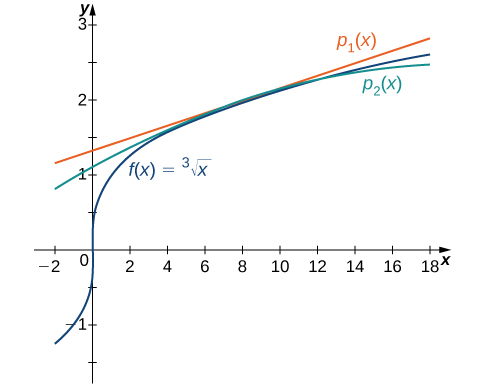
\includegraphics[scale=1]{./figures/web.jpeg}
    \end{center}
   \end{minipage}
   \bigbreak \noindent 
   Then, Using the first Taylor polynomial at $x=8$, we can estimate
    \[
    \sqrt[3]{11} \approx p_1(11) = 2 + \frac{1}{12}(11 - 8) = 2.25.
    \]
    Using the second Taylor polynomial at $x=8$, we obtain
    \[
    \sqrt[3]{11} \approx p_2(11) = 2 + \frac{1}{12}(11 - 8) - \frac{1}{288}(11 - 8)^2 = 2.21875.
    \]
    \bigbreak \noindent By Taylor’s Theorem with Remainder, there exists a $c$ in the interval $(8,11)$ such that the remainder when approximating $\sqrt[3]{11}$ by the first Taylor polynomial satisfies
    \[
    R_1(11) = \frac{f''(c)}{2!}(11 - 8)^2.
    \]
    We do not know the exact value of $c$, so we find an upper bound on $R_1(11)$ by determining the maximum value of $f''$ on the interval $(8,11)$. Since $f''(x) = -\frac{2}{9}x^{-\frac{5}{3}}$, the largest value for $|f''(x)|$ on that interval occurs at $x=8$. Using the fact that $f''(8) = -\frac{1}{144}$, we obtain
    \[
    |R_1(11)| \leq \frac{1}{144} \cdot 2!(11 - 8)^2 = 0.03125.
    \]
    Similarly, to estimate $R_2(11)$, we use the fact that
    \[
    R_2(11) = \frac{f'''(c)}{3!}(11 - 8)^3.
    \]
    Since $f'''(x) = \frac{10}{27}x^{-\frac{8}{3}}$, the maximum value of $f'''$ on the interval $(8,11)$ is $f'''(8) \approx 0.0014468$. Therefore, we have
    \[
    |R_2(11)| \leq 0.0014468 \cdot 3!(11 - 8)^3 \approx 0.0065104.
    \]

    \pagebreak 
    \begin{exm}[Approximating sin x Using Maclaurin Polynomials]
        We know the Maclaurin series for $\sin{x}$ is given by
        \begin{align*}
            &p_{2m+1} = p_{2m+2} \\
            &=x-\frac{x^{3}}{3!} + \frac{x^{5}}{5!} - \frac{x^{7}}{7!}  + ... + \frac{(-1)^{m}x^{2m+1}}{(2m+1)!}
        .\end{align*}
        For $m \in \mathbb{Z^{+}}$
        \begin{enumerate}[label=(\alph*)]
            \item Use the fifth Maclaurin polynomial for  $\sin{(x)} $ to approximate  $\sin{\left(\frac{\pi}{18}\right)} $ and bound the error. 
            \item For what values of $x$ does the fifth Maclaurin polynomial approximate  $\sin{(x)}$ to within $0.0001$?
        \end{enumerate}
    \end{exm}
    \bigbreak \noindent 
    \textit{\textcolor{red}{Solution}.}
    The fifth Maclaurin polynomial is
    \[ p_5(x) = x - \frac{x^3}{3!} + \frac{x^5}{5!}. \]
    Using this polynomial, we can estimate as follows:
    \[ \sin\left(\frac{\pi}{18}\right) \approx p_5\left(\frac{\pi}{18}\right) = \frac{\pi}{18} - \frac{1}{3!}\left(\frac{\pi}{18}\right)^3 + \frac{1}{5!}\left(\frac{\pi}{18}\right)^5 \approx 0.173648. \]
    To estimate the error, use the fact that the sixth Maclaurin polynomial is \( p_6(x) = p_5(x) \) and calculate a bound on \( R_6\left(\frac{\pi}{18}\right) \). By Uniqueness of Taylor Series, the remainder is
    \[ R_6\left(\frac{\pi}{18}\right) = \frac{f^{(7)}(c)}{7!}\left(\frac{\pi}{18}\right)^7 \]
    for some \( c \) between 0 and \( \frac{\pi}{18} \). Using the fact that \( \left|f^{(7)}(x)\right| \leq 1 \) for all \( x \), we find that the magnitude of the error is at most
    \[ \frac{1}{7!} \cdot \left(\frac{\pi}{18}\right)^7 \leq 9.8 \times 10^{-10}. \]
    We need to find the values of \( x \) such that
    \[ \frac{1}{7!}|x|^7 \leq 0.0001. \]
    Solving this inequality for \( x \), we have that the fifth Maclaurin polynomial gives an estimate to within 0.0001 as long as \( |x| < 0.907. \)

    \pagebreak 
    \phantomsection
    \addcontentsline{toc}{subsection}{Representing Functions with Taylor and Maclaurin Series}
    \subsection*{Representing Functions with Taylor and Maclaurin Series}
    \bigbreak \noindent 
    \textbf{\textcolor{red}{Remark.}} Now that we are able to bound the remainder Rn(x), we can use this bound to prove that a Taylor series for f at a converges to f.
    \bigbreak \noindent 
    We now discuss issues of convergence for Taylor series. We begin by showing how to find a Taylor series for a function, and how to find its interval of convergence.
    \begin{exm}[Finding a Taylor Series]
        Find the Taylor series for  $f(x) = \frac{1}{x} $ at  $x=1$. Determine the interval of convergence.
    \end{exm}
    \bigbreak \noindent 
    \textcolor{red}{\textit{Solution.}}
    For $f(x) = \frac{1}{x}$, the values of the function and its first four derivatives at $x=1$ are
    \[
    \begin{alignedat}{2}
        f(x) &= \frac{1}{x}, \quad \quad &&f(1) = 1, \\
        f'(x) &= -\frac{1}{x^2}, \quad \quad &&f'(1) = -1, \\
        f''(x) &= \frac{2}{x^3}, \quad \quad &&f''(1) = 2, \\
        f'''(x) &= -\frac{3 \cdot 2}{x^4}, \quad \quad &&f'''(1) = -3!, \\
        f^{(4)}(x) &= \frac{4 \cdot 3 \cdot 2}{x^5}, \quad \quad &&f^{(4)}(1) = 4!.
    \end{alignedat}
    \]
    That is, we have $f^{(n)}(1) = (-1)^n n!$ for all $n \geq 0$. Therefore, the Taylor series for $f$ at $x=1$ is given by
    \[
    \sum_{n=0}^{\infty} \frac{f^{(n)}(1)}{n!}(x-1)^n = \sum_{n=0}^{\infty} (-1)^n (x-1)^n.
    \]
    To find the interval of convergence, we use the ratio test. We find that
    \[
    \left| \frac{a_{n+1}}{a_n} \right| = \left| \frac{(-1)^{n+1}(x-1)^{n+1}}{(-1)^n(x-1)^n} \right| = |x-1|.
    \]
    Thus, the series converges if $|x-1| < 1$. That is, the series converges for $0 < x < 2$. Next, we need to check the endpoints. At $x=2$, we see that
    \[
    \sum_{n=0}^{\infty} (-1)^n (2-1)^n = \sum_{n=0}^{\infty} (-1)^n
    \]
    diverges by the divergence test. Similarly, at $x=0$,
    \[
    \sum_{n=0}^{\infty} (-1)^n (0-1)^n = \sum_{n=0}^{\infty} (-1)^{2n} = \sum_{n=0}^{\infty} 1
    \]
    diverges. Therefore, the interval of convergence is $(0,2)$.

    \pagebreak \bigbreak \noindent 
    \begin{thrmm}[Convergence of Taylor Series]
        Suppose that $f$ has derivatives of all orders on an interval $I$ containing $a$. Then the Taylor series
        \[
        \sum_{n=0}^{\infty} \frac{f^{(n)}(a)}{n!}(x-a)^n
        \]
        converges to $f(x)$ for all $x$ in $I$ if and only if
        \[
        \lim_{n \to \infty} R_n(x) = 0
        \]
        for all $x$ in $I$.
    \end{thrmm}
    
    \bigbreak \noindent 
    \begin{notebox}
        With this theorem, we can prove that a Taylor series for $f$ at $a$ converges to $f$ if we can prove that the remainder $R_n(x) \to 0$. To prove that $R_n(x) \to 0$, we typically use the bound
        \[
        |R_n(x)| \leq \frac{M}{(n+1)!}|x - a|^{n+1}
        \]
        from Taylor’s theorem with remainder.
    \end{notebox}

    \bigbreak \noindent 
    \begin{exm}
    For each of the following functions, find the Maclaurin series and its interval of convergence. Use Taylor’s Theorem with Remainder to prove that the Maclaurin series for  $f$ converges to  $f$ on that interval.    
    \begin{enumerate}[label=(\alph*)]
        \item $e^{x}$
        \item $\sin{(x)}$
    \end{enumerate}
    \end{exm}
    \bigbreak \noindent 
    \textcolor{red}{\textit{Solution (a).}}
    Using the $n$th Maclaurin polynomial for $e^x$ found in Example 6.12a., we find that the Maclaurin series for $e^x$ is given by
    \[
    \sum_{n=0}^{\infty} \frac{x^n}{n!}.
    \]
    To determine the interval of convergence, we use the ratio test. Since
    \[
    \left| \frac{a_{n+1}}{a_n} \right| = \left| \frac{x^{n+1}}{(n+1)!} \cdot \frac{n!}{x^n} \right| = |x|,
    \]
    we have
    \[
    \lim_{n \to \infty} \left| \frac{a_{n+1}}{a_n} \right| = \lim_{n \to \infty} |x| = 0
    \]
    for all $x$. Therefore, the series converges absolutely for all $x$, and thus, the interval of convergence is $(-\infty, \infty)$.
    To show that the series converges to $e^x$ for all $x$, we use the fact that $f^{(n)}(x) = e^x$ for all $n \geq 0$ and $e^x$ is an increasing function on $(-\infty, \infty)$. Therefore, for any real number $b$, the maximum value of $e^x$ for all $|x| \leq b$ is $e^b$. Thus,
    \[
    |R_n(x)| \leq \frac{e^b}{(n+1)!} |x|^{n+1}.
    \]
    Since we just showed that
    \[
    \sum_{n=0}^{\infty} \left| \frac{x^n}{n!} \right|
    \]
    converges for all $x$, by the divergence test, we know that
    \[
    \lim_{n \to \infty} \frac{|x|^{n+1}}{(n+1)!} = 0
    \]
    for any real number $x$. By combining this fact with the squeeze theorem, the result is $\lim_{n \to \infty} R_n(x) = 0$.
    \bigbreak \noindent 
    \textcolor{red}{\textit{Solution (b).}}
    Using the $n$th Maclaurin polynomial for $\sin x$ found in Example 6.12b., we find that the Maclaurin series for $\sin x$ is given by
    \[
    \sum_{n=0}^{\infty} (-1)^n \frac{x^{2n+1}}{(2n+1)!}.
    \]
    In order to apply the ratio test, consider
    \[
    \left| \frac{a_{n+1}}{a_n} \right| = \left| \frac{x^{2n+3}}{(2n+3)!} \cdot \frac{(2n+1)!}{x^{2n+1}} \right| = \left| x^2 \right| \frac{1}{(2n+3)(2n+2)}.
    \]
    Since
    \[
    \lim_{n \to \infty} \left| x^2 \right| \frac{1}{(2n+3)(2n+2)} = 0
    \]
    for all $x$, we obtain the interval of convergence as $(-\infty, \infty)$.
    To show that the Maclaurin series converges to $\sin x$, look at $R_n(x)$. For each $x$ there exists a real number $c$ between $0$ and $x$ such that
    \[
    R_n(x) = \frac{f^{(n+1)}(c)}{(n+1)!} x^{n+1}.
    \]
    Since $\left| f^{(n+1)}(c) \right| \leq 1$ for all integers $n$ and all real numbers $c$, we have
    \[
    \left| R_n(x) \right| \leq \frac{|x|^{n+1}}{(n+1)!}
    \]
    for all real numbers $x$. Using the same idea as in part a., the result is $\lim_{n \to \infty} R_n(x) = 0$ for all $x$, and therefore, the Maclaurin series for $\sin x$ converges to $\sin x$ for all real $x$.

    \pagebreak
    \phantomsection
    \addcontentsline{toc}{section}{6.4 Working with Taylor Series}
    \section*{6.4 Working with Taylor Series}
    \bigbreak \noindent 

    \phantomsection
    \addcontentsline{toc}{subsection}{The Binomial Series}
    \subsection*{The Binomial Series}
    \bigbreak \noindent 
    Our first goal in this section is to determine the Maclaurin series for the function \( f(x) = (1+x)^r \) for all real numbers \( r \). The Maclaurin series for this function is known as the binomial series. We begin by considering the simplest case: \( r \) is a nonnegative integer. We recall that, for \( r = 0, 1, 2, 3, 4 \), \( f(x) = (1+x)^r \) can be written as
    \begin{align*}
    f(x) &= (1+x)^0 = 1, \\
    f(x) &= (1+x)^1 = 1 + x, \\
    f(x) &= (1+x)^2 = 1 + 2x + x^2, \\
    f(x) &= (1+x)^3 = 1 + 3x + 3x^2 + x^3, \\
    f(x) &= (1+x)^4 = 1 + 4x + 6x^2 + 4x^3 + x^4.
    \end{align*}
    \bigbreak \noindent
    The expressions on the right-hand side are known as binomial expansions and the coefficients are known as binomial coefficients. More generally, for any nonnegative integer \( r \), the binomial coefficient of \( x^n \) in the binomial expansion of \( (1+x)^r \) is given by
    \bigbreak \noindent 
    \begin{align*}
    \binom{r}{n} &= \frac{r!}{n!(r-n)!} 
    \end{align*}
    and
    \begin{align*}
        f(x) &= (1+x)^r  \\
             &= \binom{r}{0}1 + \binom{r}{1}x + \binom{r}{2}x^2 + \binom{r}{3}x^3 + \cdots + \binom{r}{r-1}x^{r-1} + \binom{r}{r}x^r  \\
             &= \sum_{n=0} ^{r} \binom{r}{n}x^n. 
    .\end{align*}
    \bigbreak \noindent
    For example, using this formula for \( r=5 \), we see that
    \begin{align*}
    f(x) &= (1+x)^5 \\
    &= \binom{5}{0}1 + \binom{5}{1}x + \binom{5}{2}x^2 + \binom{5}{3}x^3 + \binom{5}{4}x^4 + \binom{5}{5}x^5 \\
    &= \frac{5!}{0!5!}1 + \frac{5!}{1!4!}x + \frac{5!}{2!3!}x^2 + \frac{5!}{3!2!}x^3 + \frac{5!}{4!1!}x^4 + \frac{5!}{5!0!}x^5 \\
    &= 1 + 5x + 10x^2 + 10x^3 + 5x^4 + x^5.
    \end{align*}
    \bigbreak \noindent 
    We now consider the case when the exponent \( r \) is any real number, not necessarily a nonnegative integer. If \( r \) is not a nonnegative integer, then \( f(x) = (1+x)^r \) cannot be written as a finite polynomial. However, we can find a power series for \( f \). Specifically, we look for the Maclaurin series for \( f \). To do this, we find the derivatives of \( f \) and evaluate them at \( x=0 \).
    \begin{equation}
    \begin{alignedat}{2}
        f(x) &= (1+x)^r \quad \quad &&f(0) = 1 \\
        f'(x) &= r(1+x)^{r-1}\quad \quad  &&f'(0) = r \\
        f''(x) &= r(r-1)(1+x)^{r-2} \quad \quad && f''(0) = r(r-1) \\
        f'''(x) &= r(r-1)(r-2)(1+x)^{r-3} \quad \quad &&f'''(0) = r(r-1)(r-2) \\
        f^{(n)}(x) &= r(r-1)(r-2) \cdots (r-n+1)(1+x)^{r-n} \quad \quad &&f^{(n)}(0) = r(r-1)(r-2) \cdots (r-n+1)
    \end{alignedat}
    \end{equation}
    \bigbreak \noindent
    We conclude that the coefficients in the binomial series are given by
    \[
    \frac{f^{(n)}(0)}{n!} = \frac{r(r-1)(r-2) \cdots (r-n+1)}{n!}.
    \]
    \bigbreak \noindent 
    We note that if $r$ is a nonnegative integer, then the $(r+1)$st derivative $f^{(r+1)}$ is the zero function, and the series terminates. In addition, if $r$ is a nonnegative integer, then Equation 6.8 for the coefficients agrees with Equation 6.6 for the coefficients, and the formula for the binomial series agrees with Equation 6.7 for the finite binomial expansion. More generally, to denote the binomial coefficients for any real number $r$, we define
    \begin{align*}
    \binom{r}{n} = \frac{r(r-1)(r-2)\cdots(r-n+1)}{n!}.
    \end{align*}
    \bigbreak \noindent
    With this notation, we can write the binomial series for $(1 + x)^r$ as
    \begin{align*}
    \sum_{n=0}^{\infty} \binom{r}{n} x^n = 1 + rx + \frac{r(r-1)}{2!}x^2 + \cdots + \frac{r(r-1)\cdots(r-n+1)}{n!}x^n + \cdots. \tag{6.9}
    \end{align*}
    \bigbreak \noindent
    We now need to determine the interval of convergence for the binomial series Equation 6.9. We apply the ratio test. Consequently, we consider
    \bigbreak \noindent 
    \begin{align*}
    &\frac{\left| a_{n+1} \right|}{\left| a_n \right|} = \frac{\left| r(r-1)(r-2)\cdots(r-n) \left| x \right|\right|^{n+1} }{(n+1)!} \cdot \frac{n!}{\left|r(r-1)(r-2)\cdots (r-n+1)\right|\abs{x}^{n}}  \\
    &= \frac{\left| r-n \right| \left| x \right|}{n+1}.
    \end{align*}
    \bigbreak \noindent
    Since
    \begin{align*}
    \lim_{n \to \infty} \frac{\left| a_{n+1} \right|}{\left| a_n \right|} = \left| x \right| < 1
    \end{align*}
    if and only if $\left| x \right| < 1$, we conclude that the interval of convergence for the binomial series is $(-1,1)$. The behavior at the endpoints depends on $r$. It can be shown that for $r \geq 0$ the series converges at both endpoints; for $-1 < r < 0$, the series converges at $x = 1$ and diverges at $x = -1$; and for $r < -1$, the series diverges at both endpoints. The binomial series does converge to $(1 + x)^r$ in $(-1,1)$ for all real numbers $r$, but proving this fact by showing that the remainder $R_n(x) \to 0$ is difficult.
    \bigbreak \noindent 
    Since
    \begin{align*}
        \lim_{n \to \infty} \left| \frac{a_{n+1}}{a_n} \right| = |x| < 1
    \end{align*}
    if and only if \(|x| < 1\), we conclude that the interval of convergence for the binomial series is \((-1,1)\).
    \bigbreak \noindent
    The behavior at the endpoints depends on \(r\). It can be shown that for \(r \geq 0\) the series converges at both endpoints; for \(-1 < r < 0\), the series converges at \(x = 1\) and diverges at \(x = -1\); and for \(r < -1\), the series diverges at both endpoints. The binomial series does converge to \((1+x)^r\) in \((-1,1)\) for all real numbers \(r\), but proving this fact by showing that the remainder \(R_n(x) \to 0\) is difficult.

    \bigbreak \noindent 
    \begin{dfn}[Binomial Series]
        For any real number \(r\), the Maclaurin series for \( f(x) = (1 + x)^r \) is the binomial series. It converges to \(f\) for \(|x| < 1\), and we write
        \begin{align*}
            (1 + x)^r = \sum_{n=0}^{\infty} \binom{r}{n} x^n = 1 + rx + \frac{r(r-1)}{2!}x^2 + \cdots + \frac{r(r-1) \cdots (r-n+1)}{n!}x^n + \cdots
        \end{align*}
        for \(|x| < 1\).
    \end{dfn}

    \pagebreak 
    \begin{exm}[Finding Binomial Series]
        \bigbreak \noindent 
        \begin{enumerate}[label=(\alph*)]
            \item Find the binomial series for \( f(x) = \sqrt{1 + x} \).
            \item Use the third-order Maclaurin polynomial \( p_3(x) \) to estimate \( \sqrt{1.5} \). Use Taylor’s theorem to bound the error. Use a graphing utility to compare the graphs of \( f \) and \( p_3 \).
        \end{enumerate}
    \end{exm}
    \bigbreak \noindent 
    \textcolor{red}{\textit{Solution.}}
    Here \( r = 12 \).
    \bigbreak \noindent
    Using the definition for the binomial series, we obtain
    \begin{align*}
    \sqrt{1+x} &= 1 + \frac{1}{2}x + \frac{(1/2)(-1/2)}{2!}x^2 + \frac{(1/2)(-1/2)(-3/2)}{3!}x^3 + \cdots \\
    &= 1 + \frac{1}{2}x - \frac{1}{2!}\frac{1^2}{2}x^2 + \frac{1}{3!}\frac{1\cdot 3}{2^3}x^3 - \cdots + (-1)^{n+1}\frac{1}{n!}\frac{1\cdot 3 \cdot 5 \cdots (2n-3)}{2^n}x^n + \cdots \\
    &= 1 + \sum_{n=1}^{\infty} (-1)^{n+1}\frac{1}{n!}\frac{1\cdot 3 \cdot 5 \cdots (2n-3)}{2^n}x^n.
    \end{align*}
    \bigbreak \noindent 
    From the result in part a. the third-order Maclaurin polynomial is
    \begin{align*}
    p_3(x) &= 1 + 12x - 18x^2 + \frac{1}{16}x^3.
    \end{align*}
    \bigbreak
    \noindent Therefore,
    \begin{align*}
    \sqrt{1.5} &= 1 + \sqrt{0.5} \approx 1 + \frac{1}{2}(0.5) - \frac{18}{2}(0.5)^2 + \frac{1}{16}(0.5)^3 \approx 1.2266.
    \end{align*}
    \bigbreak
    \noindent From Taylor's theorem, the error satisfies
    \begin{align*}
    R_3(0.5) &= \frac{f^{(4)}(c)}{4!}(0.5)^4
    \end{align*}
    \bigbreak
    \noindent for some $c$ between $0$ and $0.5$. Since $f^{(4)}(x) = -\frac{1524}{(1+x)^{7/2}}$, and the maximum value of $\left| f^{(4)}(x) \right|$ on the interval $(0,0.5)$ occurs at $x=0$, we have
    \begin{align*}
    \left| R_3(0.5) \right| &\leq \frac{15}{4!}\frac{24}{(0.5)^4} \approx 0.00244.
    \end{align*}
    \bigbreak
    \noindent The function and the Maclaurin polynomial $p_3$ are

    \pagebreak 
    \phantomsection
    \addcontentsline{toc}{subsection}{Common Functions Expressed as Taylor Series}
    \subsection*{Common Functions Expressed as Taylor Series}
    \bigbreak \noindent 
    \begin{center}
        
    \begin{tabular}{|c|c|c|}
    \hline
    Function & Maclaurin Series & Interval of Convergence \\ \hline
    $f(x) = \frac{1}{1 - x}$ & $\sum_{n=0}^{\infty} x^n$ & $-1 < x < 1$ \\ \hline
    $f(x) = e^x$ & $\sum_{n=0}^{\infty} \frac{x^n}{n!}$ & $-\infty < x < \infty$ \\ \hline
    $f(x) = \sin x$ & $\sum_{n=0}^{\infty} (-1)^n \frac{x^{2n+1}}{(2n+1)!}$ & $-\infty < x < \infty$ \\ \hline
    $f(x) = \cos x$ & $\sum_{n=0}^{\infty} (-1)^n \frac{x^{2n}}{(2n)!}$ & $-\infty < x < \infty$ \\ \hline
    $f(x) = \ln(1 + x)$ & $\sum_{n=1}^{\infty} (-1)^{n+1} \frac{x^n}{n}$ & $-1 < x \leq 1$ \\ \hline
    $f(x) = \tan^{-1} x$ & $\sum_{n=0}^{\infty} (-1)^n \frac{x^{2n+1}}{2n+1}$ & $-1 \leq x \leq 1$ \\ \hline
    $f(x) = (1 + x)^r$ & $\sum_{n=0}^{\infty} \binom{r}{n} x^n$ & $-1 < x < 1$ \\ \hline
    \end{tabular}
    \end{center}

    \bigbreak \noindent 
    \begin{exm}[Deriving Maclaurin Series from Known Series]
        Find the Maclaurin series of each of the following functions by using one of the series listed in Table 6.1.
        \begin{enumerate}[label=(\alph*)]
            \item $f(x) = \cos{(x)} $
            \item $f(x) = \sinh{(x)} $
        \end{enumerate}
    \end{exm}
    \bigbreak \noindent 
    \textcolor{red}{\textit{Solution.}}
    Using the Maclaurin series for $\cos x$, we find that the Maclaurin series for $\sqrt{\cos x}$ is given by
    \begin{align*}
        &\sum_{n=0}^{\infty} \frac{(-1)^n (\sqrt{x})^{2n}}{(2n)!} = \sum_{n=0}^{\infty} \frac{(-1)^n x^n}{(2n)!}  \\
        &= 1 - \frac{x}{2!} + \frac{x^2}{4!} - \frac{x^3}{6!} + \frac{x^4}{8!} - \cdots.
    .\end{align*}
    \bigbreak \noindent
    This series converges to $\sqrt{\cos x}$ for all $x$ in the domain of $\sqrt{\cos x}$; that is, for all $x \geq 0$.
    \bigbreak \noindent 
    To find the Maclaurin series for $\sinh x$, we use the fact that
    \[
    \sinh x = \frac{e^x - e^{-x}}{2}.
    \]
    \bigbreak \noindent
    Using the Maclaurin series for $e^x$, we see that the $n$th term in the Maclaurin series for $\sinh x$ is given by
    \[
    \frac{x^n}{n!} - \frac{(-x)^n}{n!}.
    \]
    \bigbreak \noindent
    For $n$ even, this term is zero. For $n$ odd, this term is $\frac{2x^n}{n!}$. Therefore, the Maclaurin series for $\sinh x$ has only odd-order terms and is given by
    \[
    \sum_{n=0}^{\infty} \frac{x^{2n+1}}{(2n+1)!} = x + \frac{x^3}{3!} + \frac{x^5}{5!} + \cdots.
    \]

    \pagebreak 
    \begin{exm}[Differentiating a Series to Find a New Series]
        Use the binomial series for $\sqrt{1+x}$ to find the binomial series for $\frac{1}{\sqrt{1+x}} $ 
        
    \end{exm}
    \bigbreak \noindent 
    \textcolor{red}{\textit{Solution.}}
    \bigbreak
\noindent The two functions are related by
\begin{align*}
\frac{d}{dx}\sqrt{1+x} = \frac{1}{2\sqrt{1+x}},
\end{align*}
so the binomial series for $\frac{1}{\sqrt{1+x}}$ is given by
\begin{align*}
\frac{1}{\sqrt{1+x}} = 2 \frac{d}{dx}\sqrt{1+x} = 1 + \sum_{n=1}^{\infty} \frac{(-1)^n}{n!} \frac{1 \cdot 3 \cdot 5 \cdots (2n-1)}{2^n} x^n.
\end{align*}
\bigbreak \noindent 
    



    






    
    









    

    





    



    
    
    
    
    
    


    
    
    
    


\end{document}
